\renewcommand*{\arraystretch}{1.1}

\noindent\begin{tabularx}{17cm}{|p{1.95cm}|X|}
	\hline
	workload    & BI \\ \hline
%
	query       & 25 \\ \hline
%
	title       & Weighted paths \\ \hline
%
    pattern     & \hfill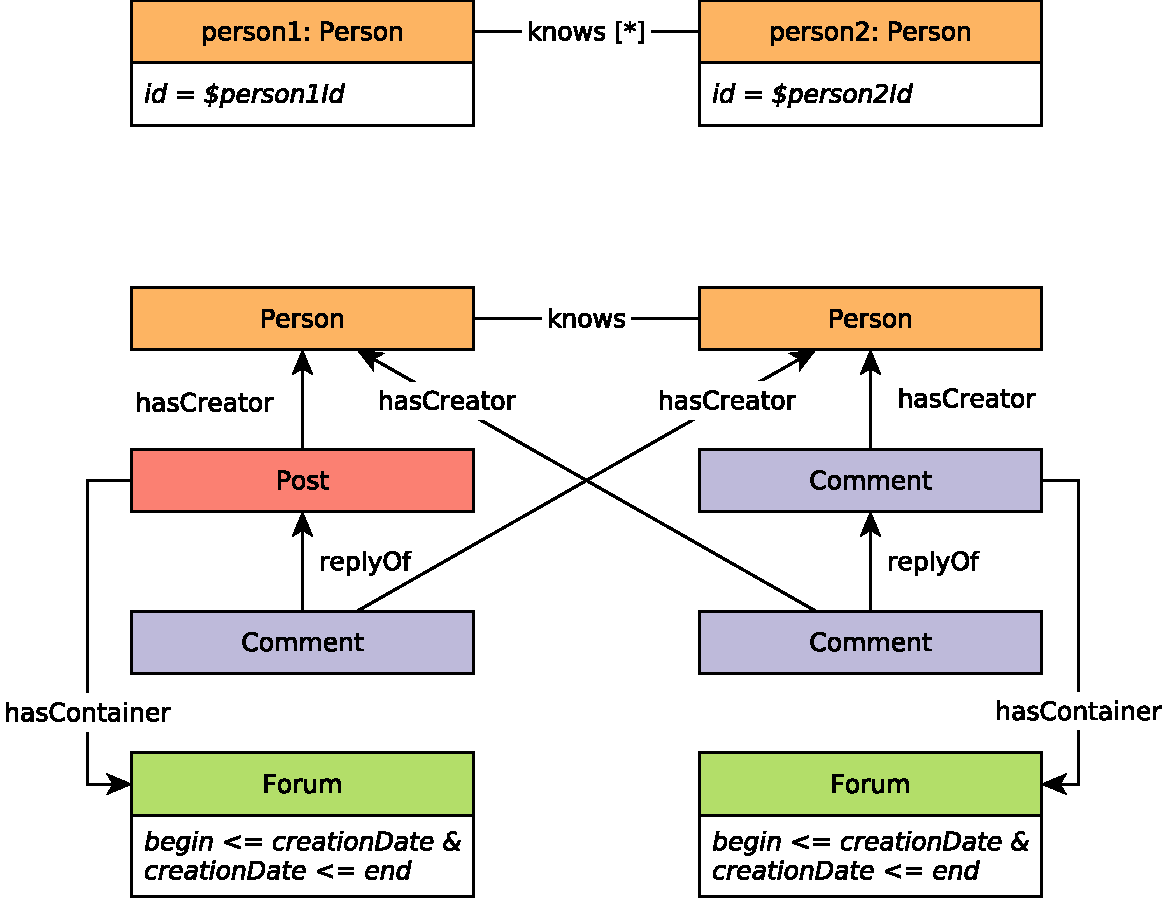
\includegraphics[scale=\patternscale,margin=0cm .2cm]{patterns/bi-read-25}\hfill\vadjust{} \\ \hline
%
	description & Given two Persons, find all (unweighted) shortest paths between these
two Persons, in the subgraph induced by the Knows relationship.

Then, for each path calculate a weight. The nodes in the path are
Persons, and the weight of a path is the sum of weights between every
pair of consecutive Person nodes in the path.

The weight for a pair of Persons is calculated such that every reply (by
one of the Persons) to a Post (by the other Person) contributes 1.0, and
every reply (by ones of the Persons) to a Comment (by the other Person)
contributes 0.5.

Only consider messages that were created in a forum that was created
within the timeframe \texttt{{[}startDate,\ endDate{]}}.

Return all the paths with shortest length, and their weights.
 \\ \hline
%
	
%
	parameters  &
	\vspace{1.1ex}{\begin{tabularx}{14.2cm}{|c|M|m{2cm}|Y|} \hline
	\cellcolor{black!70} \color{white} $\mathsf{1}$ & \varname{person1Id} & \cellcolor{gray!20} \vartype{64-bit Integer} &  \\ \hline
	\cellcolor{black!70} \color{white} $\mathsf{2}$ & \varname{person2Id} & \cellcolor{gray!20} \vartype{64-bit Integer} &  \\ \hline
	\cellcolor{black!70} \color{white} $\mathsf{3}$ & \varname{startDate} & \cellcolor{gray!20} \vartype{Date} &  \\ \hline
	\cellcolor{black!70} \color{white} $\mathsf{4}$ & \varname{endDate} & \cellcolor{gray!20} \vartype{Date} &  \\ \hline
	\end{tabularx}}\vspace{1.1ex} \\ \hline
%
	
	result      &
	\vspace{1.1ex}{\begin{tabularx}{14.2cm}{|c|M|m{2cm}|Y|} \hline
	\cellcolor{black!70} \color{white} $\mathsf{1}$ & \varname{person.id} & \cellcolor{gray!20} \vartype{64-bit Integer} & Identifiers representing an ordered sequence of the Persons in the path weight \\ \hline
	\end{tabularx}}\vspace{1.1ex} \\ \hline
	
%
	sort        &
	\vspace{1.1ex}{\begin{tabular}{|c|l|c|} \hline
	\cellcolor{black!70} \color{white} $\mathsf{1}$ & \varname{weight} & \cellcolor{gray!20} $\desc$ \\ \hline
	\end{tabular}}\vspace{1.1ex} \\ \hline
	%
	%
	choke points &
	\multicolumn{1}{>{\raggedright}l|}{
	  \chokepoint{1.2}, 
	  \chokepoint{2.1}, 
	  \chokepoint{2.2}, 
	  \chokepoint{2.4}, 
	  \chokepoint{3.3}, 
	  \chokepoint{5.1}, 
	  \chokepoint{5.3}, 
	  \chokepoint{7.2}, 
	  \chokepoint{7.3}
	  } \\ \hline
	%
\end{tabularx}
\vspace{2ex}